\documentclass[12pt]{article}
\usepackage[paper=letterpaper,margin=1.5cm]{geometry}
\usepackage{amsmath}
\usepackage{amssymb}
\usepackage{amsfonts}
\usepackage{mathtools}
%\usepackage[utf8]{inputenc}
%\usepackage{newtxtext, newtxmath}
\usepackage{lmodern}     % set math font to Latin modern math
\usepackage[T1]{fontenc}
\renewcommand\rmdefault{ptm}
%\usepackage{enumitem}
\usepackage[shortlabels]{enumitem}
\usepackage{titling}
\usepackage{graphicx}
\usepackage[colorlinks=true]{hyperref}
\usepackage{setspace}
\usepackage{subfigure} 
\usepackage{braket}
\usepackage{color}
\usepackage{tabularx}
\usepackage[table]{xcolor}
\usepackage{listings}
\usepackage{mathrsfs}
\usepackage{stackengine}
\usepackage{physics}
\usepackage{afterpage}
\usepackage{pdfpages}
\usepackage[export]{adjustbox}
\usepackage{biblatex}

\setstackEOL{\\}

\definecolor{dkgreen}{rgb}{0,0.6,0}
\definecolor{gray}{rgb}{0.5,0.5,0.5}
\definecolor{mauve}{rgb}{0.58,0,0.82}


\lstset{frame=tb,
  language=Python,
  aboveskip=3mm,
  belowskip=3mm,
  showstringspaces=false,
  columns=flexible,
  basicstyle={\small\ttfamily},
  numbers=none,
  numberstyle=\tiny\color{gray},
  keywordstyle=\color{blue},
  commentstyle=\color{dkgreen},
  stringstyle=\color{mauve},
  breaklines=true,
  breakatwhitespace=true,
  tabsize=3
}
\setlength{\droptitle}{-6em}

\makeatletter
% we use \prefix@<level> only if it is defined
\renewcommand{\@seccntformat}[1]{%
  \ifcsname prefix@#1\endcsname
    \csname prefix@#1\endcsname
  \else
    \csname the#1\endcsname\quad
  \fi}
% define \prefix@section
\newcommand\prefix@section{}
\newcommand{\prefix@subsection}{}
\newcommand{\prefix@subsubsection}{}
\renewcommand{\thesubsection}{\arabic{subsection}}
\makeatother
\DeclareMathOperator*{\argmin}{argmin}
\newcommand{\partbreak}{\begin{center}\rule{17.5cm}{2pt}\end{center}}
\newcommand{\alignbreak}{\begin{center}\rule{15cm}{1pt}\end{center}}
\newcommand{\tightalignbreak}{\vspace{-5mm}\alignbreak\vspace{-5mm}}
\newcommand{\hop}{\vspace{1mm}}
\newcommand{\jump}{\vspace{5mm}}
\newcommand{\R}{\mathbb{R}}
\newcommand{\C}{\mathbb{C}}
\newcommand{\N}{\mathbb{N}}
\newcommand{\G}{\mathbb{G}}
\renewcommand{\S}{\mathbb{S}}
\newcommand{\bt}{\textbf}
\newcommand{\xdot}{\dot{x}}
\renewcommand{\star}{^{*}}
\newcommand{\ydot}{\dot{y}}
\newcommand{\lm}{\mathrm{\lambda}}
\renewcommand{\th}{\theta}
\newcommand{\id}{\mathbb{I}}
\newcommand{\si}{\Sigma}
\newcommand{\Si}{\si}
\newcommand{\inv}{^{-1}}
\newcommand{\T}{^\intercal}
\renewcommand{\tr}{\text{tr}}
\newcommand{\ep}{\varepsilon}
\newcommand{\ph}{\varphi}
%\renewcomand{\norm}[1]{\left\lVert#1\right\rVert}
\definecolor{cit}{rgb}{0.05,0.2,0.45}
\addtolength{\jot}{1em}
\newcommand{\solution}[1]{

\noindent{\color{cit}\textbf{Solution:} #1}}

\newcounter{tmpctr}
\newcommand\fancyRoman[1]{%
  \setcounter{tmpctr}{#1}%
  \setbox0=\hbox{\kern0.3pt\textsf{\Roman{tmpctr}}}%
  \setstackgap{S}{-.9pt}%
  \Shortstack{\rule{\dimexpr\wd0+.1ex}{.9pt}\\\copy0\\
              \rule{\dimexpr\wd0+.1ex}{.9pt}}%
}

\newcommand{\Id}{\fancyRoman{2}}

% Enter the specific assignment number and topic of that assignment below, and replace "Your Name" with your actual name.
\title{STAT 31410: Homework 1}
\author{Caleb Derrickson}
\date{October 17, 2023}

\begin{document}
\onehalfspacing
\maketitle

{\color{cit}\vspace{2mm}\noindent\textbf{Collaborators:}} The TA's of the class, as well as Kevin Hefner, Alexander Cram, and Steven Lee.

\tableofcontents

\newpage

\section{Problem 1}
Determine for which values of $\beta > 0$ there is ``finite-time blow-up" of solutions(i.e. there exists a finite $T > 0$ such that lim$_{t \rightarrow T}$ $\lvert x(t) \rvert = \ + \infty$) for the following scalar ode:
\[
\dot{x} = x^\beta, \hspace{3mm} x(0) = x_0 \in \R^+.
\]

Specify the domain of existence of the solution, i.e. determine $T$ as a function of $x_0$ and $\beta$.

\partbreak
\begin{solution}

Treating this as a separable ODE, we can apply the following:

\alignbreak
\begin{align}
&\dot{x} = x^\beta &\text{(Given.)} \nonumber\\
&\frac{dx}{dt} = x^\beta &\text{(Explicit form of $\dot{x}$.)} \nonumber\\
&\frac{dx}{x^\beta} = dt &\text{(Rearranging.)} \nonumber\\        
\int_{x_0}^x &\frac{dx'}{(x')^\beta} = \int_0^t dt' &\text{(Integrating with given bounds.)} \label{pb1:cases}
\end{align}
\alignbreak

From \ref{pb1:cases}, we run into an immediate issue concerning $\beta$. Since the solution for $\beta = 1$ will have a different structure than other valid $\beta$, we can break \ref{pb1:cases} into three cases, depending on its value with respect to 1.

\newpage
\underline{\textbf{Case 1:}} $\beta > 1$

Then, 
\begin{align}
 &\int_{x_0}^x \frac{dx'}{(x')^\beta} = \int_0^t dt' &\text{(Given.)}\nonumber\\
 &\frac{1}{1 - \beta}(x')^{1 - \beta}\bigg|_{x_0}^x = t' \bigg|_0^t &\text{(Integrating.)}\nonumber\\
&x^{1 - \beta} = (1 - \beta)t + x_0^{1 - \beta} &\text{(Applying bounds and Rearranging.)} \nonumber\\
&x = \sqrt[1 - \beta]{(1 - \beta)t + x_0^{1 - \beta}} &\text{(Simplifying.)}\nonumber\\
&x = \frac{1}{\sqrt[\beta - 1]{(1 - \beta)t + x_0^{1 - \beta}}} &\text{(Applying reciprocal.)} \nonumber
\end{align}

Note the last step was performed with the mind that $1 - \beta < 0$. Since $t \geq 0, (1 - \beta)t \leq 0$, while $x_0^{1 - \beta}$ is strictly positive. Thus there will be some time T where these two quantities will equal, making the denominator zero, and $x$ blow up as a result. This will happen explicitly when
\[T = \frac{1}{1 - \beta}\Bigg(\frac{1}{x_0^{\beta - 1}}\Bigg)\]

\underline{\textbf{Case 2:}} $\beta = 1$

Then,
\begin{align}
     &\int_{x_0}^x \frac{dx'}{x'} = \int_0^t dt' &\text{(Given with $\beta = 1$.)}\nonumber\\
    &\ln{x} - \ln x_0 = t &\text{(Integrating and applying bounds.)}\nonumber\\
    &x(t) = x_0e^t &\text{(Rearranging and simplifying.)}\nonumber\\
\end{align}

Since our solution is an exponential in $t$, there will be no finite time $T$ such that $x(t)$ ``blows up".

\newpage
\underline{\textbf{Case 3:}} $0 < \beta < 1$

Then,
\begin{align}
    &\int_{x_0}^x \frac{dx'}{(x')^\beta} = \int_0^t dt' &\text{(Given.)}\nonumber\\
    &\frac{1}{1 - \beta}(x')^{1 - \beta}\bigg|_{x_0}^x = t' \bigg|_0^t &\text{(Integrating.)}\nonumber\\
    &x^{1 - \beta} = (1 - \beta)t + x_0^{1 - \beta} &\text{(Applying bounds and Rearranging.)} \nonumber\\
    &x = \sqrt[1 - \beta]{(1 - \beta)t + x_0^{1 - \beta}} &\text{(Simplifying.)}\nonumber
\end{align}

Note that $0 < \beta < 1$, i.e. $1 - \beta > 0$. Thus, $(1 - \beta)t$ is strictly positive, as is $x_0^{1 - \beta}$. Thus there is no time such that $x(t)$ ``blows up".

\alignbreak

Therefore, it has been shown the only case where there is a finite time in which $x(t)$ ``blows up" is when $\beta > 1$. In this case, a finite time $T$ was found for which the solution ``blows up". Any other values of $\beta$, i.e. $\beta \in (0, 1]$, gave solutions where there were no finite times in which our solution blows up.

\jump
\end{solution}% End of problem 1 part 1

\newpage
\subsection{Problem 1, part 2}
In the remainder of this problem, let's focus on $\beta = 2$  and $x_0 = 1$. What is the time $T$ to ``blow up" in this case? Introduce the following transformation from $t$ to a new time variable $\tau$:
\[
\tau = \int_0^t 1 + x^2(s) ds, \hspace{3mm} t\in [0,T)
\]
where $x(s)$ satisfies the original problem $dx/ds = x^2$. Show that this is a one-to-one mapping between $t \in [0, T)$ and $\tau$, and specify the range of $\tau$. Let $y(\tau) = x(t(\tau))$; what differential equation does $y(\tau)$ satisfy? Does $y(\tau)$ have finite time blow-up? 

\partbreak
\begin{solution}

    We are given $\beta = 2, x_0 = 1$. From the first case of problem 1, we have
    \[
    x = \frac{1}{1 - t}, \hspace{10mm} T = \frac{1}{2 - 1}\Bigg(\frac{1}{1^{2 - 1}}\Bigg) = 1
    \]

    Since we have an explicit function for $x(t)$, we can plug this in to find $\tau$.

    \alignbreak
    \begin{align}
        \tau &= \int_0^{t} 1 + \frac{1}{(1 - t')^2}dt' &\text{(Plugging in $x(t)$.)}\nonumber\\
        &= \int_0^{t} \frac{(1 - t')^2 + 1}{(1 - t')^2}dt' &\text{(Simplifying.)}\nonumber\\
        &= \int_1^{1-t} \frac{u^2 + 1}{u^2} du &\text{($u$ sub. with $u = 1 - t'$.)} \nonumber\\
        &= \ u\bigg|_1^{1 - t} + \frac{1}{u}\bigg|^1_{1 - t} &\text{(Integrating.)}\nonumber\\
        &= 1 - t - 1 + 1 - \frac{1}{1 - t} &\text{(Applying bounds.)}\nonumber\\
        &= t + 1 - \frac{1}{1-t} &\text{(Simplifying.)}\nonumber\\
        &= \frac{(1 - t)^2 - 1}{1 - t} &\text{(Simplifying.)}\nonumber\\
        \tau&= \frac{t(t - 2)}{1 - t} &\text{(Simplifying.)} \label{p1:tau in t}
    \end{align}
    \alignbreak

    By \ref{p1:tau in t}, we have an explicit function for $\tau$ in terms of $t$. To show injectivity, it suffices to show that $\tau'(t) > 0$ for all $t > 0$.

    \begin{center}\rule{15cm}{0.5pt}\end{center}
    \begin{align}
        \frac{d\tau}{dt} &= \frac{d}{dt}\bigg[ t + 1 - \frac{1}{1 - t}\bigg] &\text{(Third to last line above.)}\nonumber\\
        &= 1 + \frac{1}{(1 - t)^2} &\text{(Differentiating.)} \label{p1:diff}
    \end{align}
    \alignbreak
    We can note that \ref{p1:diff} is strictly positive for all $t > 0$, thus $\tau$ is injective.

    Next, we wish to show what differential equation does $y(\tau)$ satisfy. Note that from the lectures, $y(\tau)$ should satisfy
    \[\frac{dy}{d\tau} = F(y) = \frac{f(y)}{1 + |f(y)|}\]

    From the chain rule,
    \[\frac{dy}{d\tau} = \frac{dx}{dt}\frac{dt}{d\tau}\]

    We have an explicit form for $dx/dt$, and we have the reciprocal for $dt/d\tau$. Thus, we will simply flip $d\tau/dt$ to get $dt/d\tau$. The following steps can thus be justified:

    \newpage
    \alignbreak
    \begin{align}
        \frac{d\tau}{dt} &= \frac{(1 - t)^2 + 1}{(1 - t)^2} \nonumber\\
        \frac{dt}{d\tau} &= \frac{(1 - t)^2}{(1 - t)^2 + 1} \label{p1:dtdtau}\\  
        \frac{dx}{dt} &= \frac{d}{dt}\Bigg[ \frac{1}{1 - t}\Bigg] = \frac{1}{(1 - t)^2} \label{p1:dxdt}\\
        \frac{dy}{d\tau} &= \frac{dx}{dt}\frac{dt}{d\tau} &\text{(Given.)}\nonumber\\
        &= \Bigg(\frac{1}{(1 - t)^2}\Bigg)\Bigg( \frac{(1 - t)^2}{(1 - t)^2 + 1}\Bigg) &\text{(Plugging in \ref{p1:dxdt} and \ref{p1:dtdtau}.)}\nonumber\\
        &= \frac{1}{(1 - t)^2 + 1} &\text{(Simplifying.)}\nonumber\\
        &= \frac{\frac{1}{(1 - t)^2}}{1 + \frac{1}{(1 - t)^2}} &\text{(Dividing by $(1 - t)^2$.)}\nonumber\\
        &= \frac{y^2}{1 + y^2} &\text{(Applying $y(\tau) = x(t(\tau))$.)}\nonumber\\
        \frac{dy}{d\tau} &= \frac{f(y)}{1 + |f(y)|} &\text{($f(y) = y^2$.)}\nonumber
    \end{align}
    \alignbreak

    With initial condition $y(\tau = 0) = x(t = 0) = 1$. Since $y(\tau) = x(t(\tau))$ with $x = \frac{1}{1 - t}$, there will only be finite time blow up when $t(\tau) = 1$. Note we have $\tau(t)$, given as \ref{p1:tau in t}. We can investigate \ref{p1:tau in t} to surmise any issues which may arise in $t(\tau)$. \ref{p1:tau in t} takes in $t \in (1, \infty)$. Within this interval, \ref{p1:tau in t} lies above $\tau = 1$, so we can gesture there will be no such point where $t(\tau) = 1$, therefore no finite time blow up will occur. 
\end{solution}% End of problem 1 part 2

\newpage

\section{Problem 2}
Consider the scalar initial value problem
\begin{align}
    \dot{x} = -|x|^\beta, \hspace{5mm} x(0) = 0. \label{p2:ODE}
\end{align}

For which values of $\beta > 0$ is the solution $x(t) = 0$ guaranteed to be unique on some interval $J = [-a, a], \ a > 0$? If there is no such guarantee, explicitly construct a family of solutions to the initial value problem on the interval $J$.   
\partbreak

\begin{solution}

    For the sake of completion, I will include the theorem I will be invoking below:

    \alignbreak
    \begin{quote}
            Suppose there are constants $a, b, > 0$ such that $f:B_b(x_0) \rightarrow \R^n$ is Lipschitz with constant $k \geq 1$. Then our initial value problem \ref{p2:ODE} has a unique solution $x(t)$ for $t \in J = [-a, a]$ provided $a < b/M$, where $M = \max \{|f(x)| : x \in B_b(x_0)\}.$
    \end{quote}
    \alignbreak

    For any $x \in B_b(x_0) = B_b(0)$, $x^\beta \leq b^\beta$. Then $M = \max \{|f(x)| : x \in B_b(0)\} = b^\beta$. We have a bound on $a$ which depends on $b$, i.e. $a < b/M$. Plugging in what we found for $M$ implies $a < b^{1 - \beta}$. Thus we have three cases, which will yield different intervals on which the solution $x(t) = 0$ is guaranteed unique. Note in each case given we are seeking a $b$ which will give us an upper bound on $a$.

    \jump
    \underline{\textbf{Case 1:}} $\beta > 1$. 
    \jump
    
    If $\beta > 1$, then $a < \frac{1}{b^\beta}$. Since $b > 0$ by the theorem, any choice of $b$ will give us a valid bound for $a$, so $J = [-a, a]$ is finite, thus properly defined. 

    \jump
    \underline{\textbf{Case 2:}} $0 < \beta < 1$.
    \jump
    
    In this case, we run into a problem where our function $f(x) = -|x|^\beta$ is not Lipschitz continuous. to prove this, it suffices to show the derivative of $f(x)$ is not bounded. 
    \newpage
    \alignbreak
    \begin{align}
        f'(x) &= \frac{d}{dx}\Big[ -|x|^\beta \Big] &\text{(Given.)}\nonumber\\
        &= -\beta|x|^{\beta - 1} \cdot \frac{|x|}{x} &\text{(Taking derivative.)}\nonumber\\
        &= -\frac{\beta\text{sgn}(x)}{|x|^{1 - \beta}} &\text{(Defintition of sgn(x) and simplifying.)}
    \end{align}
    \alignbreak

    Thus as $x \rightarrow 0^+$, $f'(x) \rightarrow -\infty$, therefore $f'(x)$ is not bounded, meaning we cannot find a constant $k$ for Lipschitz continuity. Thus there is no bound for $a$ which $x(t) = 0$ is guaranteed unique.

    \jump
    To find a family of solutions for this ODE, we just need to solve it. I claim that the following solution $x(t)$ solves \ref{p2:ODE} for any choice of $\alpha > 0$.

    \begin{align}
        x(t) = 
        \Bigg\{\begin{array}{lr}
             0, &t < \alpha\\
             -[(t - \alpha)(1 - \beta)]^{\frac{1}{1 - \beta}}, &t \geq \alpha
        \end{array}
        \label{p2: ooa soln}
    \end{align}

    I will show below it satisfies the ODE only when $t \geq \alpha$. The case for $t < \alpha$ is obvious. 
    \alignbreak
    \begin{align}
        \frac{dx}{dt} &= \frac{d}{dx}\Bigg[ -[ (t - \alpha)(1 - \beta)] ^{\frac{1}{1-\beta}}\Bigg] &\text{(Given.)}\nonumber\\
        &= -\frac{(1 - \beta)(t - \alpha)^{\frac{1}{1 - \beta}}}{(1 - \beta)(t - \alpha)}   &\text{(Taking derivative.)}\nonumber\\
        &= -\frac{x}{x^{1 - \beta}} &\text{(Simplifying.)}\nonumber\\
        &= -|x|^\beta &\text{(Simplifying.)}\nonumber
    \end{align}
    \alignbreak
    
    Thus, \ref{p2: ooa soln} solves the system. Now we just need to show $x(t = 0) = 0$ for any choice of $\alpha > 0$. We are free to chose any $\alpha$, so if $t < \alpha$, then the initial conditions hold immediately. So \ref{p2: ooa soln} is a solution to our differential equation for any $\alpha > 0$. This is then our family of solutions in this case.  

    \newpage
    \jump
    \underline{\textbf{Case 3:}} $\beta = 1$.
    \jump

    For this case, we have $a < b^{0} = 1$, so $a \in (0, 1]$ will give us a unique solution, any $a$ outside this interval will not guarantee the uniqueness of $x(t) = 0$ on $J = [-a, a]$. We can then find a family of solutions in solving \ref{p2:ODE}. Since this is a nonlinear ordinary differential equation, it will be slightly tricky to find a solution $x(t)$. I will provide the steps below before running into a problem.
    \alignbreak
    \begin{align}
        &\dot{x} = - |x| &\text{(Given.)}\nonumber\\
        &\frac{dx}{|x|} = dt    &\text{(Assuming Separability.)}\nonumber\\
        &-\frac{x\ln |x|}{|x|} = t + C  &\text{(Integrating both sides.)}\nonumber\\
        &-\text{sgn}(x)\ln |x| = t + C   &\text{(Signature function definition.)}\nonumber\\
        &|x|^{-\text{sgn}(x)} = Ce^t &\text{(Raising both sides by $e$.)}\nonumber
    \end{align}
    \alignbreak

    If we stop here and try to apply the initial conditions, we get $0^{-1}$, which is undefined. So we are not guaranteed solutions, but the family of solutions is just the singleton set $\{0\}$.
\end{solution}

\newpage
\section{Problem 3}
 Short response: what role (if any) does the Lipschitz constant $K$ play in proving (local) existence and uniqueness of solutions of initial value problems of the form

\[
\dot{\textbf{x}} = \textbf{f}(\textbf{x}), \hspace{5mm} x(0) = x_0 \in \R^n, \hspace{5mm} \textbf{f} : \R^n \rightarrow \R^n 
\]

\partbreak
\begin{solution}

    For existence, we only require continuity, so the Lipschitz constant does not play a role here. For uniqueness, the Lipschitz constant comes into play in the coefficient of the contraction mapping $Ka = c$ in the contraction mapping theorem. I will note here there are additional proofs which don't rely on the Lipschitz constant, but the one provided to us in class does rely on it.    
\end{solution}

\newpage
\section{Problem 4}
Often in applications, the dynamics of a system being modeled, may be governed by quite different processes in different regions of the state space. And this might lead to a dynamical system that is set-wise defined, e.g.

    \begin{align}
        \dot{\textbf{x}} = 
        \Bigg\{\begin{array}{lr}
             \textbf{f}^+(x), &\sigma(\textbf{x}) > 0\\
             \textbf{f}^-(x), &\sigma(\textbf{x}) < 0
        \end{array}
        \label{p4: set dynamical system}
    \end{align}

    where the scalar equation $\sigma(x) = 0$ defines the boundary between different of state space governed by different dynamics (Note that I didn’t say anything about the dynamics for points \textbf{in} the boundary).
 
    \jump
    In the following, you explore how various possible definitions of the dynamics in the boundary might impact the behavior of the system. Specifically, consider \ref{p4: set dynamical system} with $\textbf{f}^\pm(\textbf{x})$ given as a planar, linear vector field

    \[
    \textbf{f}^\pm (\textbf{x}) = \begin{pmatrix}
         -1 \pm x_2\\
         x_2 \mp x_1
    \end{pmatrix},
    \]

    and let the boundary be defined by $\sigma(x) = x_2$.

\subsection{Problem 4, part a}
Plot the phase portrait associated with $\dot{\textbf{x}} = \textbf{f}^+(\textbf{x})$ and $\dot{\textbf{x}} = \textbf{f}^-(\textbf{x})$ , separately in the square region $x_1, x_2 \in [-2, 2]$, i.e. don’t restrict them to their regions $x_2 > 0$ or $x_2 < 0$.

\partbreak
\begin{solution}
    I will provide the code below, followed by the generated plots. I have also noted the equilibrium points of both vector fields, at $(1, \pm1)$, respectively. 
    \jump
    
\begin{lstlisting}
import numpy as np 
import matplotlib.pyplot as plt 

#constants
bound = 2 #Plotting bounds for x and y axis
# Meshgrid 
x, y = np.meshgrid(np.linspace(-bound, bound, 20),  
                   np.linspace(-bound, bound, 20)) 

#Vector directions for f plus and f minus
uplus = -1 + y
vplus = y - x
umin = -1 - y
vmin = x + y

fig, axs = plt.subplots(2, 1, figsize =(12, 12))


# Plotting Vector Field  
axs[0].quiver(x, y, uplus, vplus, color='g') 
axs[0].set_title('f^-(x)') 
axs[0].grid(True)
axs[0].scatter([1], [1], color = 'g')
axs[0].annotate("Equilibrium", (1.05, 1.05))

# Plotting Vector Field  
axs[1].quiver(x, y, umin, vmin, color='g') 
axs[1].set_title('f^+(x)') 
axs[1].grid(True)
axs[1].scatter([1], [-1], color = 'g')
axs[1].annotate("Equilibrium", (1.05, -0.95))

# Setting x, y boundary limits 
plt.xlim(-bound, bound) 
plt.ylim(-bound, bound) 
  
# show plot
plt.show() 
\end{lstlisting}

\jump
\begin{figure}[!ht]
\centering
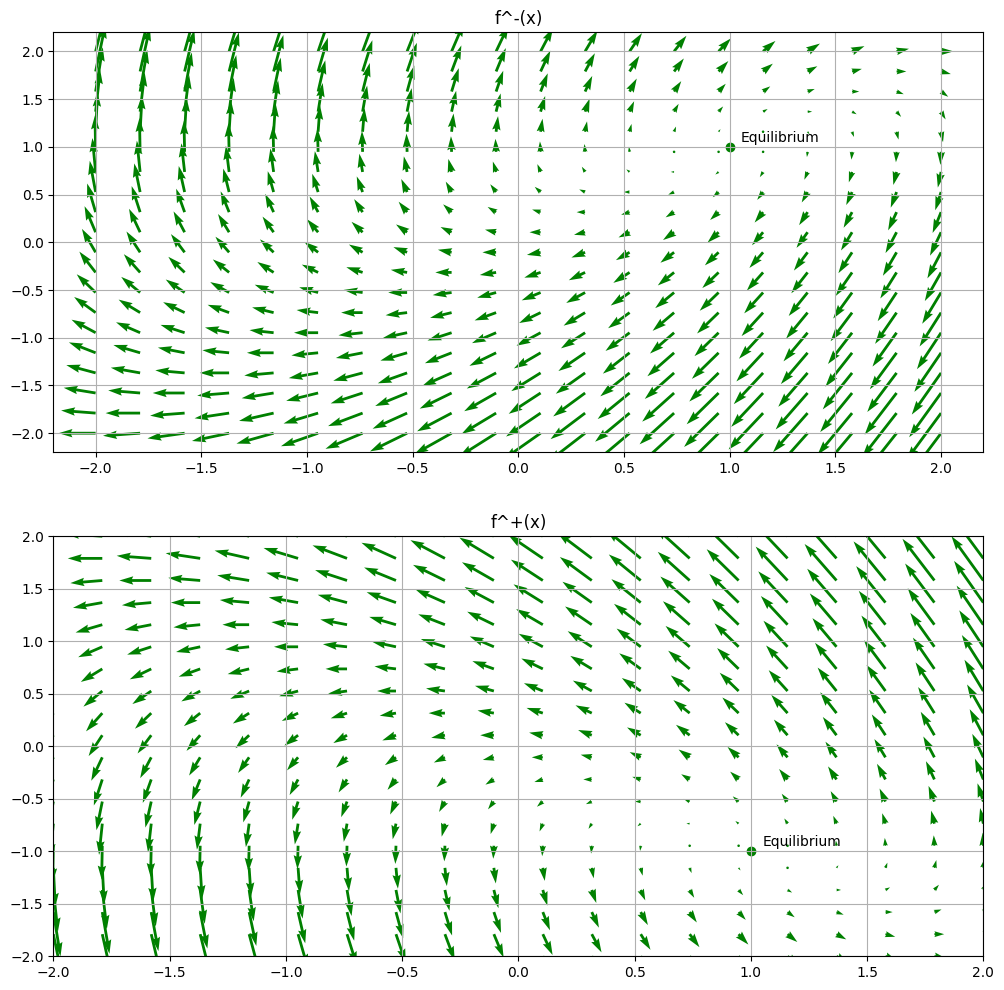
\includegraphics[scale = 0.6]{Images/individual vector fields.png}
\caption{Vector fields for $f^+$ and $f^-$ respectively.}
\label{png:individual vector fields}
\end{figure}
\end{solution}

\vspace{\floatsep}
\clearpage

\newpage
\subsection{Problem 4, part b}
Show that the vector field is discontinuous on $x_2 = 0$, so we can’t expect solutions with
initial values ($x_1$, 0) to be unique.

\partbreak
\begin{solution}
I will show this analytically, as well as numerically. To begin, recall the definition of the direcitonal derivative in direction \textbf{v}:

\alignbreak
\begin{align}
    \nabla_\textbf{v} f(\textbf{x}) := \lim_{h \rightarrow 0} \frac{\textbf{f}(\textbf{x} + h\textbf{v}) - \textbf{f}(\textbf{x})}{h} \label{p4b: directional derivative def}
\end{align}
\alignbreak

We will show we get two different directions at the boundary $(x_2 = 0)$. Thus we shall break this into two cases, where we will take the directional derivate at a point $\textbf{x} = (a, 0)$, and in direction $\textbf{v} = (0, x_2)$ where both signs will depend on the case.

\jump
\underline{\textbf{Case 1:}} $a, x_2 > 0$.
\jump

In this case, we are above the boundary, which means our system $\dot{\textbf{x}} = \textbf{f}^+(\textbf{x})$. Then, the following hold:

\alignbreak
\begin{align}
    &\textbf{x} + h\textbf{v} &= \begin{pmatrix} a\\hx_2\end{pmatrix}\nonumber\\
    &\textbf{f}^+(\textbf{x} + h\textbf{v}) - \textbf{f}^+(\textbf{x}) &= \begin{pmatrix} hx_2\\ hx_2\end{pmatrix}\nonumber\\
    \implies &\lim_{h \rightarrow 0} \frac{\textbf{f}^+(\textbf{x} + h\textbf{v}) - \textbf{f}^+(\textbf{x})}{h} &= x_2\begin{pmatrix}1\\1\end{pmatrix}\nonumber
\end{align}
\alignbreak

This should hold for any $x_2 > 0$.

\newpage
\jump
\underline{\textbf{Case 2:}} $a, x_2 < 0$.
\jump

In this case, we are below the boundary, which means our system $\dot{\textbf{x}} = \textbf{f}^-(\textbf{x})$. Then, the following hold:

\alignbreak
\begin{align}
    &\textbf{x} + h\textbf{v} &= \begin{pmatrix} a\\hx_2\end{pmatrix}\nonumber\\
    &\textbf{f}^-(\textbf{x} + h\textbf{v}) - \textbf{f}^-(\textbf{x}) &= \begin{pmatrix} -hx_2\\ hx_2\end{pmatrix}\nonumber\\
    \implies &\lim_{h \rightarrow 0} \frac{\textbf{f}^-(\textbf{x} + h\textbf{v}) - \textbf{f}^-(\textbf{x})}{h} &= x_2\begin{pmatrix}-1\\1\end{pmatrix}\nonumber
\end{align}
\alignbreak

This should hold for any $x_2 < 0$. Upon inspection, we see different directions in which our derivative is heading. If we take $x_2 \rightarrow 0$ in both cases, we see a discontinuity depending on the cases above.

\jump
In the numerical approach, we can plot these two vector fields together and notice the discontinuity along the boundary $x_2 = 0$. The code is given below, followed by the generated plots.

\begin{lstlisting}
import numpy as np 
import matplotlib.pyplot as plt 

#Trying to get a combination of the two filed onto the same plot.
xpos, ypos= np.meshgrid(np.linspace(-bound, bound, 20),  
                   np.linspace(0 , bound, 10)) 
xmin, ymin= np.meshgrid(np.linspace(-bound, bound, 20),  
                   np.linspace(-bound, 0, 10)) 

#Update vector fields
#Vector directions for f plus and f minus
uplus = -1 + ypos
vplus = ypos - xpos
umin = -1 - ymin
vmin = xmin + ymin

fig, axs = plt.subplots(1, 1, figsize =(12, 12))

# Plotting Vector Field with QUIVER 
axs.quiver(xpos, ypos, uplus, vplus, color='g') 
axs.quiver(xmin, ymin, umin, vmin, color='g') 
axs.set_title('Total Vector field') 
axs.grid(True)
axs.scatter([1, 1], [1, -1], color = 'g')
axs.annotate("Equilibrium", (1.05, 1.05))
axs.annotate("Equilibrium", (1.05, -0.95))
axs.set_xlabel("x1")
axs.set_ylabel("x2")
# Setting x, y boundary limits 
plt.xlim(-bound, bound) 
plt.ylim(-bound, bound) 
  
# Show plot with grid 
 
plt.show() 
\end{lstlisting}


\jump
\begin{figure}[!ht]
\centering
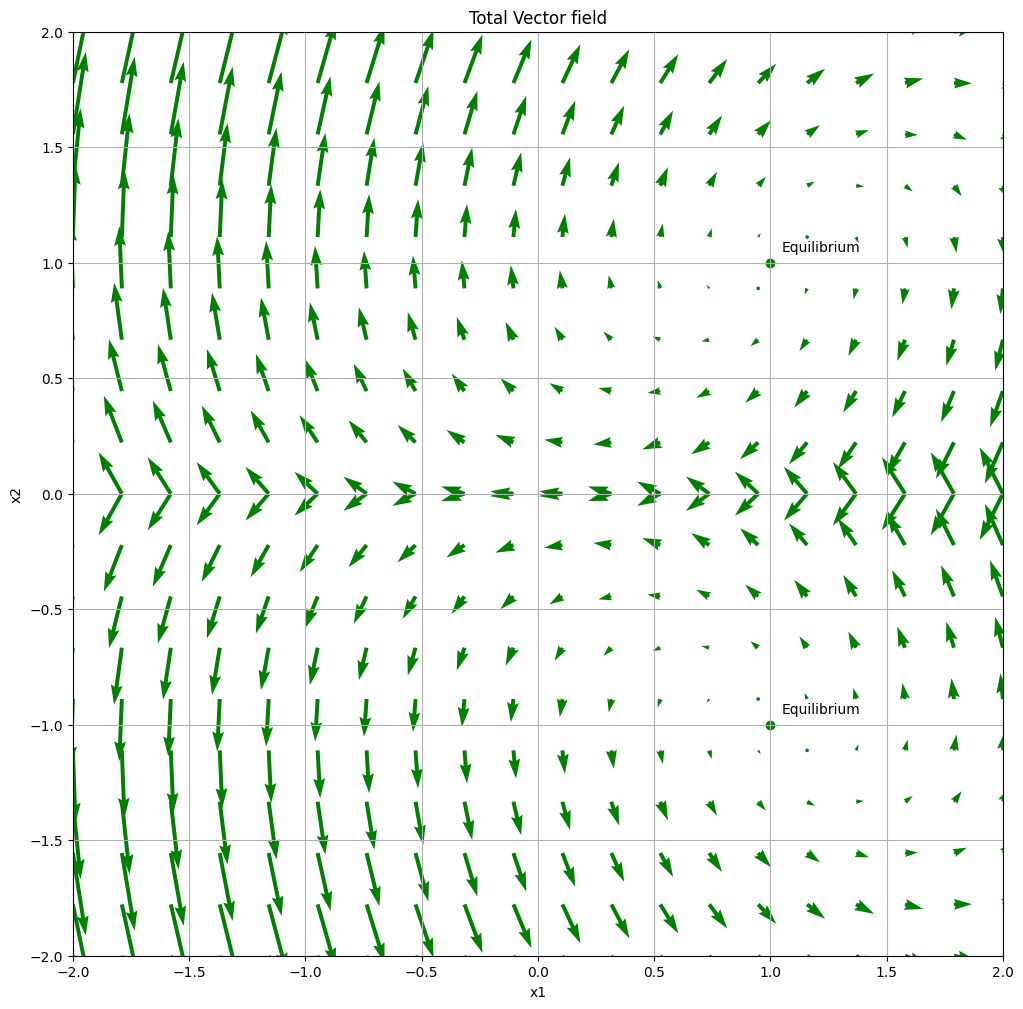
\includegraphics[scale = 0.6]{Images/vector field for system.png}
\caption{The entire Vector Field for problem 4. Note the discontinuity along the boundary $x_2 = 0$.}
\label{png:vectorfield}
\end{figure}
\end{solution}

\vspace{\floatsep}
\clearpage

\subsection{Problem 4, part c}

Let’s proceed by restricting to consideration of the forward time behavior of the model with some prescribed dynamics on the discontinuity boundary. For example, one natural way that the dynamics might be defined is as a convex combination of $f^+$ and $f^-$, i.e. let

\[
\dot{\textbf{x}} = \alpha\textbf{f}^+(\textbf{x}) + (1 - \alpha)\textbf{f}^-(\textbf{x}), \hspace{3mm} \alpha \in [0, 1], \hspace{3mm} \text{ for \textbf{x} satisfying $\sigma(\textbf{x}) = 0$}
\]

For the following choices of $\alpha$, plot the forward solution in the phase plane for an initial condition $(x_1, x_2) = (2, 1)$. (This can be done as a somewhat qualitative sketch.) (i) $\alpha = 0$, (ii) $\alpha = 0.5$, (iii) $\alpha = 1$. Comment on whether the behavior is sensitive to the choice of the parameter $\alpha \in [0, 1]$.


\partbreak

\begin{solution}

    I will describe the solution for each value of $\alpha$ first, followed by some qualitative plots. If we consider our initial conditions to be $(x_1, x_2) = (1, 2)$, then we need not worry about encountering either equilibrium of the system on our journey to the boundary. Since we have $x_2 > 0$, we are in the ``positive" regime, i.e. the vector field is spinning in a clockwise direction about the equilibrium point $(x_1, x_2) = (1, 1)$. Our approach and eventual contact with the boundary will not depend on our values of $\alpha$. Once we hit the boundary above, the solution will ``slide along" the $x_2$ axis until we reach the origin. From here, the trajectory of the solution will depend on the value for $\alpha$.

    \jump
    If $\alpha = 0$, then our boundary almost acts as an extension of the vector filed below, causing the solution to wander into the ``negative" regime in a counter clockwise manner until hitting the boundary again. This behavior will repeat for any future span of time. If $\alpha = 0.5$, then our boundary acts neither like the negative nor positive regime. In this scenario, the horizontal components of $\textbf{f}^+$ and $\textbf{f}^-$ cancel, leaving only the vertical component of each vector field. This will cause the solution to follow the $x_2$ axis for any future time. If $\alpha$ = 1, our boundary will act almost as an extension to the positive regime, mirroring the $\alpha = 0$ case. Note that for the cases of $\alpha = 0, 1$ will we have our solution ``captured" by the system (I put \textit{captured} in quotes since our vector field extends to infinity in each axis, so there will never be a point in which we leave the influence of the vector field. Our solution will not spend its time around either equilibrium point, hence my use of the word \textit{captured}). 
    
    \jump
    A qualitative plot will be provided below. This is an admittedly bad plot, since I am showing that for each successive approach along the boundary will hit at the exact same time (for $\alpha = 0, 1$) and will be sped up to the exact same speed. This is not the case, as I would expect this system would experience chaotic activity (meaning the nature of the solution will wildly vary depending on initial conditions).
\end{solution}

\jump
\begin{figure}[!ht]
\centering
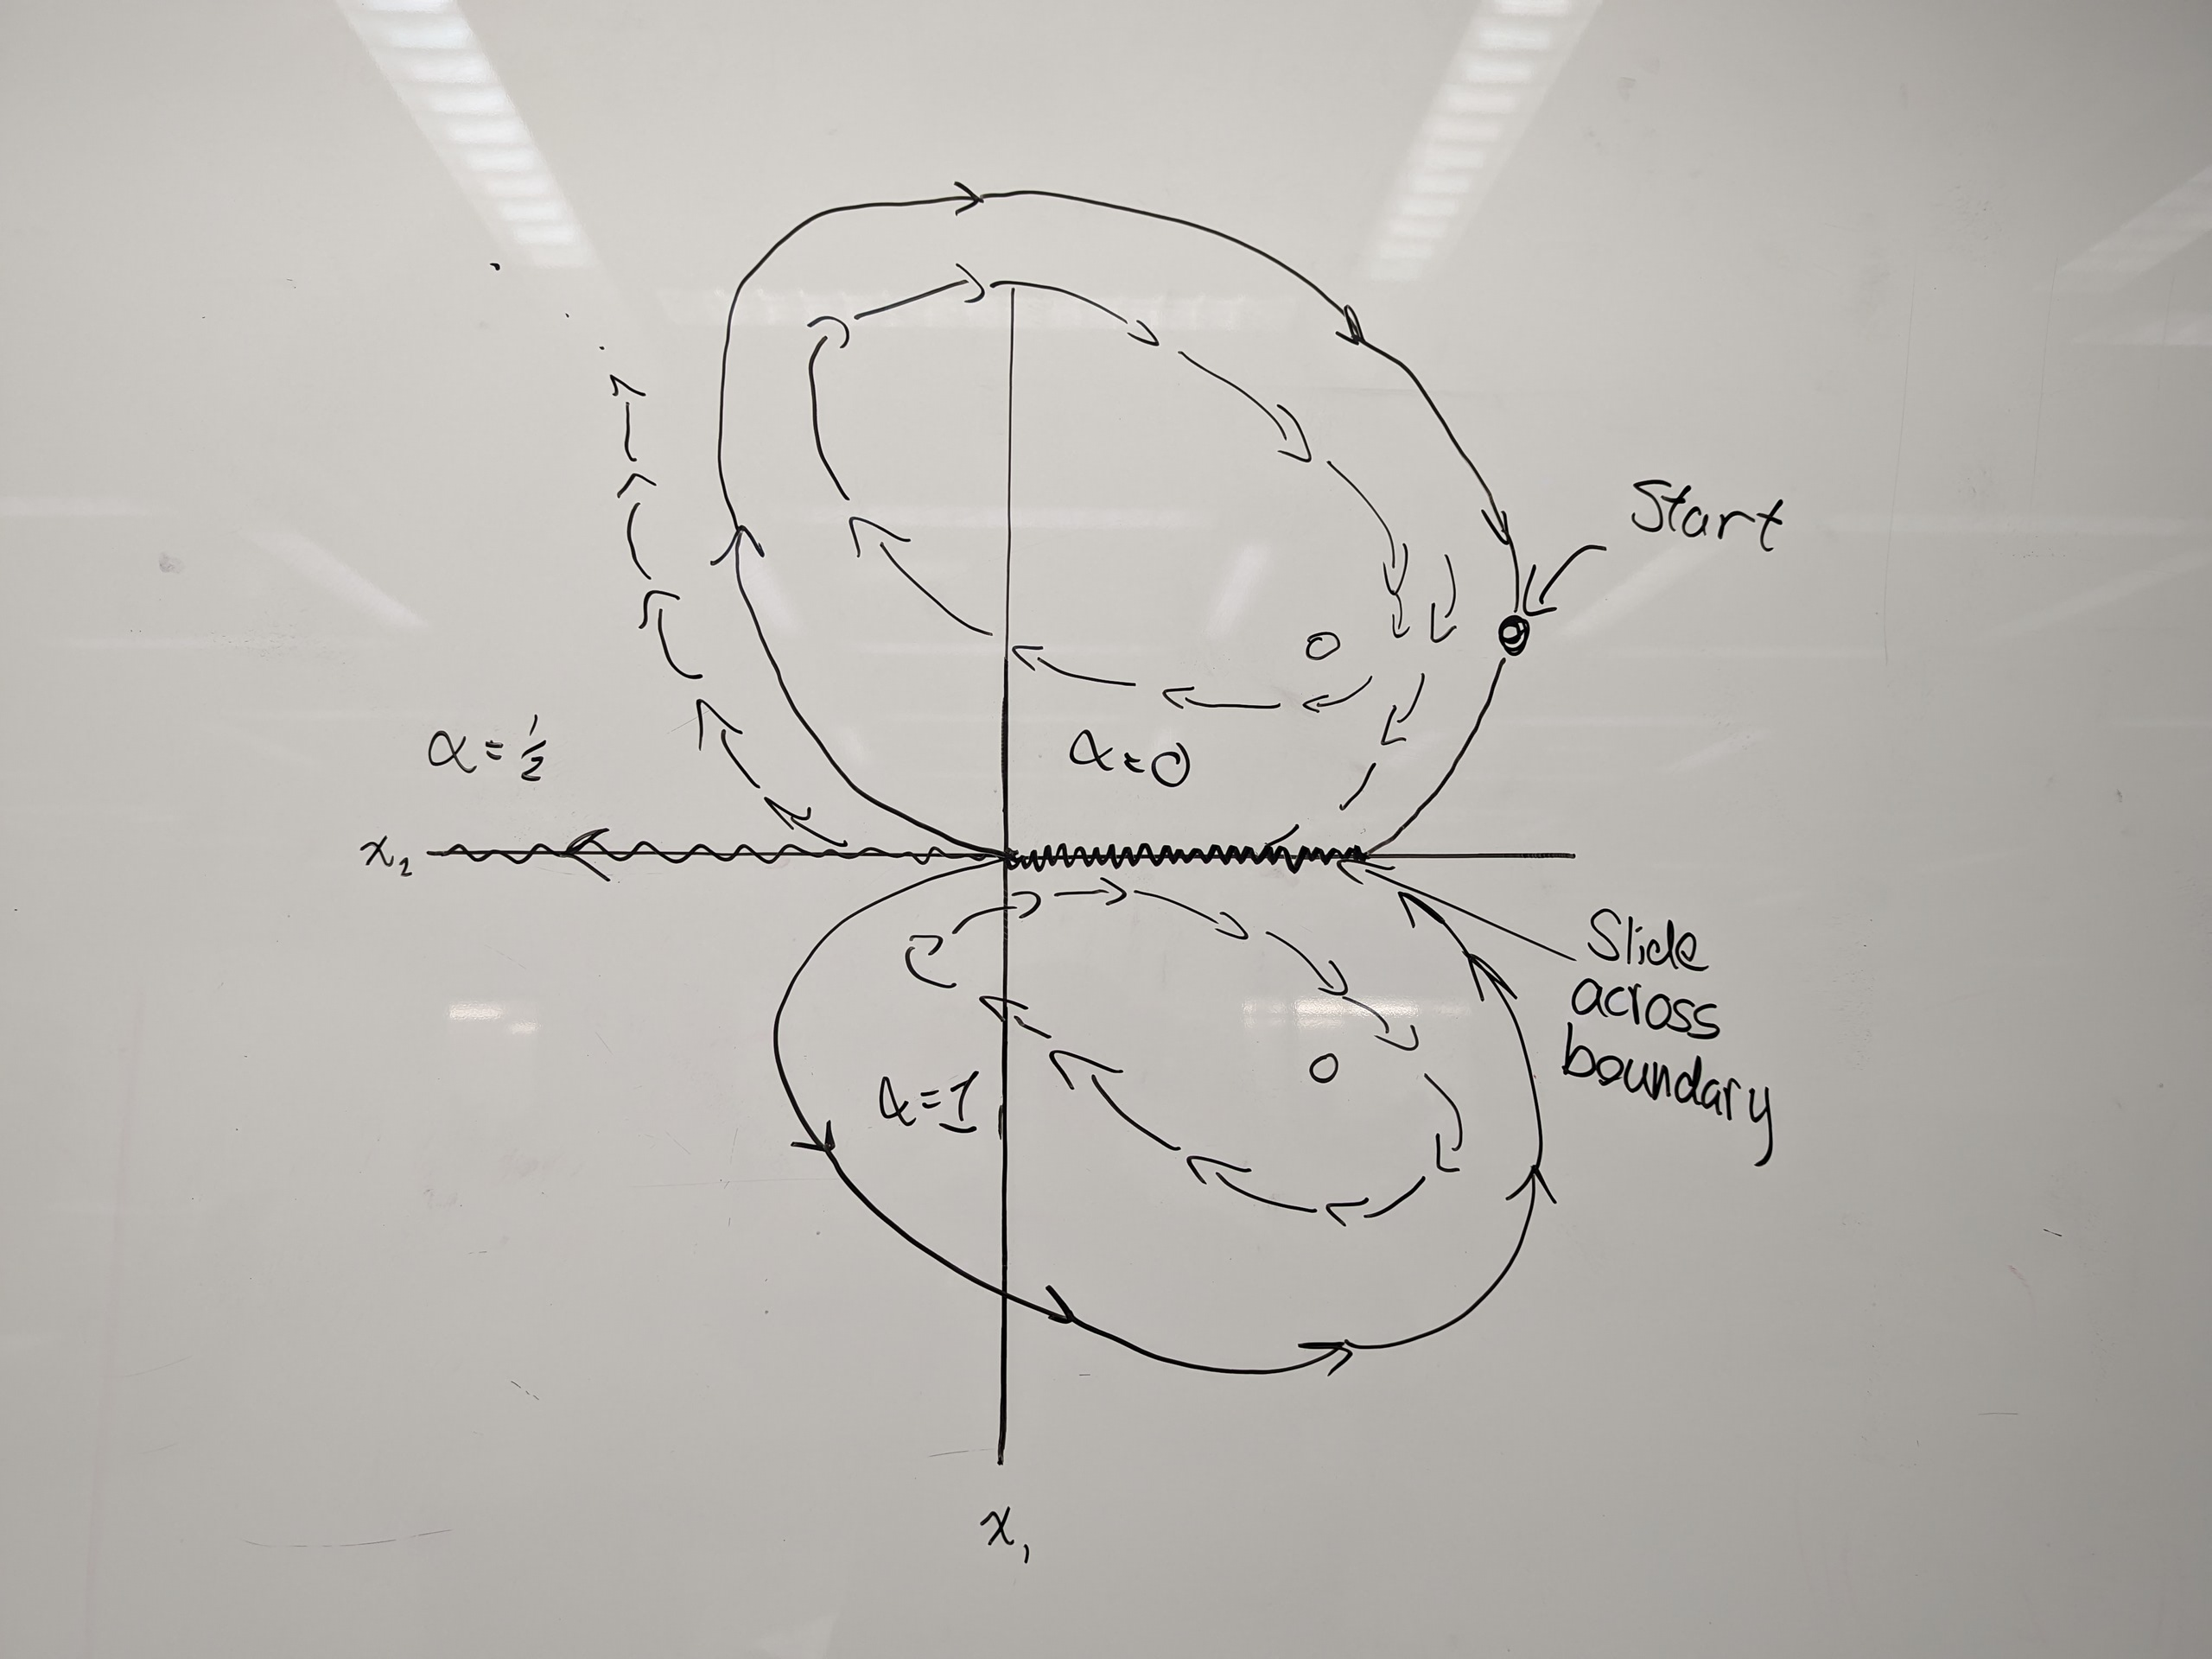
\includegraphics[width = 0.9\textwidth]{Images/qualitative plot.jpg}
\caption{A qualitative plot for the solution of our system for $\alpha = 0, 0.5, 1$. This is a really bad drawing. }
\label{png:qualitativeplot}
\end{figure}


\vspace{\floatsep}
\clearpage

\newpage
\section{Problem 5}
The following are examples of more open-ended questions, related to problem 4, and you are encouraged to explore at lease one of them, and/or pose and answer your own:

\partbreak
\begin{solution}

    I went on a slight tangent coming into this problem. Due to my lack of experience in drawing vector fields, I wanted to see an accurate representation of our system, and not me just giving it my best shot. This led me to trying to solve the system itself, given some initial conditions not knowing this was problem 5. The results I got were somewhat difficult to resolve with my intuition, but fit comfortably after re-evaluation. I will explain below, dispersing my plots when relevant, then once that's done I will include my code.

    \jump
    My initial guess to represent a boundary was to actually include an interval of $\pm \ep$ around $x_2 = 0$. From there I took the convex combination of both vector fields and noticed something interesting for fixed $\alpha$. I started with $\ep = 0.01$, which is an understandable value (I tried implementing $\ep = 0$, part c, but it seemed my program would run forever, so I omitted this). I noticed that the solution will stay on the side of the initial condition for some time, then will revert to following the expected behavior for given $\alpha$. Figure \ref{png:othervectorfield} shows this behavior.
    
    \jump
    \begin{figure}[!ht]
    \centering
    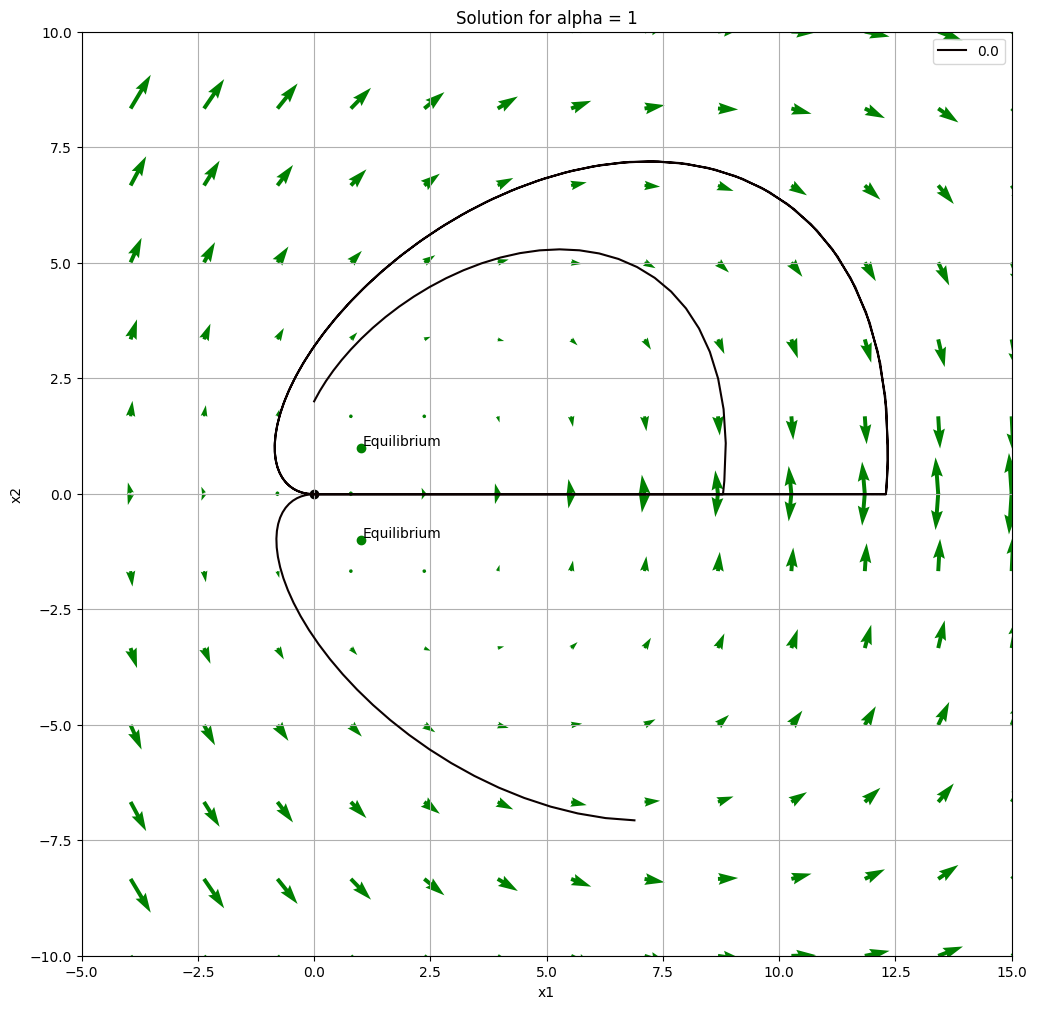
\includegraphics[width = 0.5\textwidth]{Images/small ep other vector field.png}
    \caption{A solution for $\ep = 0.01$ and $\alpha = 1$. Note for later times the solution shoots into the other field.}
    \label{png:othervectorfield}
    \end{figure}
    
    
    \vspace{\floatsep}
    \clearpage

    From there, I decided to increase the value for $\ep$, thus increasing the size of the boundary. for increasing $\ep$, not only did my code run faster, but the solution immediately goes to its expected field and slowly increases the period of, what I will call orbits. I increased $\ep$ to 0.1 to observe this behavior. My intuition is that when increasing the height of the boundary, the solution experiences the intended vector field longer, thus biasing it to the intuitively correct side. Since it experiences the vector field longer, its orbit increases ever so slightly each time it hits the boundary, thus the cycle repeats. I have included Figure \ref{png:increasing orbit} to describe this behavior.
    
    \jump
    \begin{figure}[!ht]
    \centering
    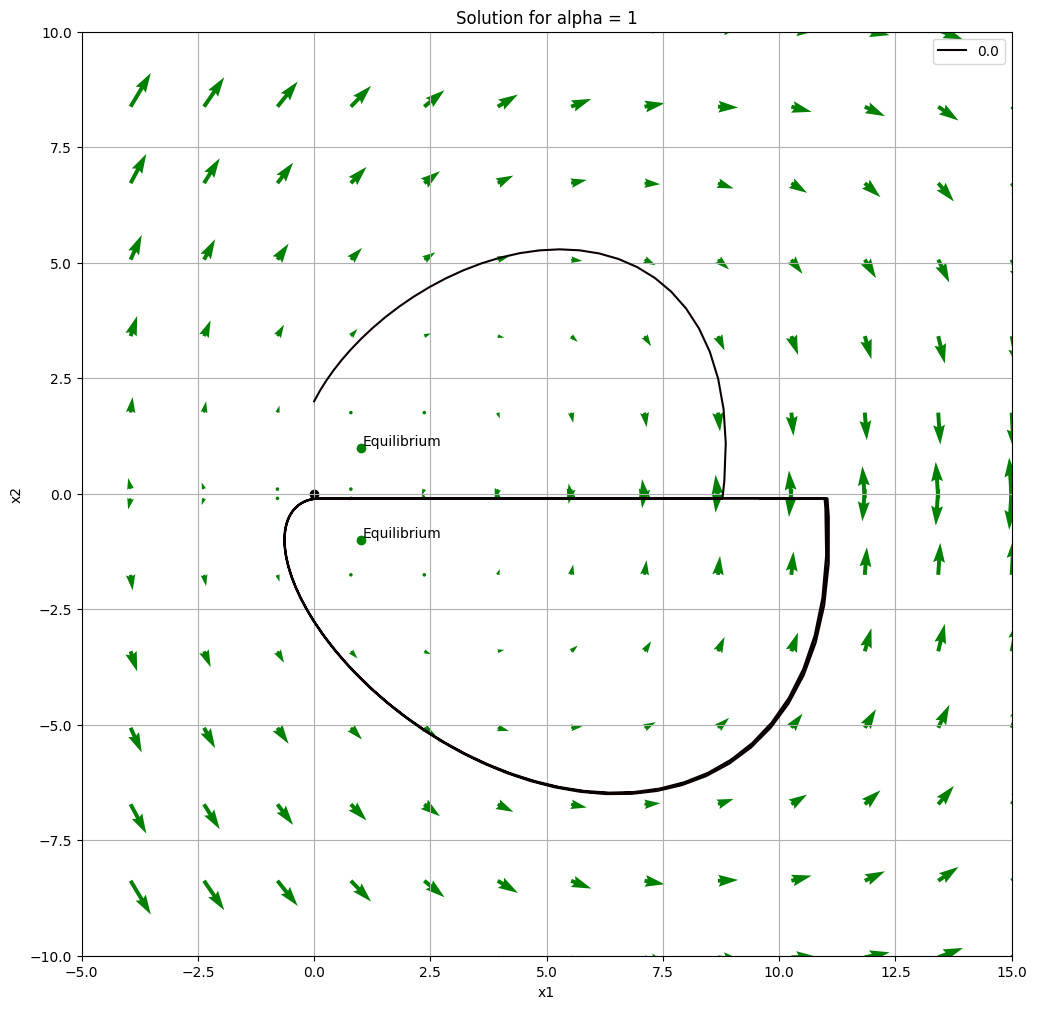
\includegraphics[width = 0.5\textwidth]{Images/longer orbits.png}
    \caption{A solution for $\ep = 0.1$ and $\alpha = 1$. Note the slightly increasing orbit.}
    \label{png:increasing orbit}
    \end{figure}

    \vspace{\floatsep}
    \clearpage

    Since this is a system which should experience some chaotic activity, I thought it necessary to investigate the system for various initial conditions. Note that I wanted to keep the system in a somewhat tight configuration, which means I will only be shifting the $x_2$ coordinate. I feel as though this should be enough for the system. It seems that there is \textit{some} changes in orbit when perturbing the initial conditions - over a longer time scale I would imagine to see more noticeable differences. I increased $\ep$ to 0.15 in Figure \ref{png:initial conditions} so we could see a larger differences in orbits. 

    \jump
    \begin{figure}[!ht]
    \centering
    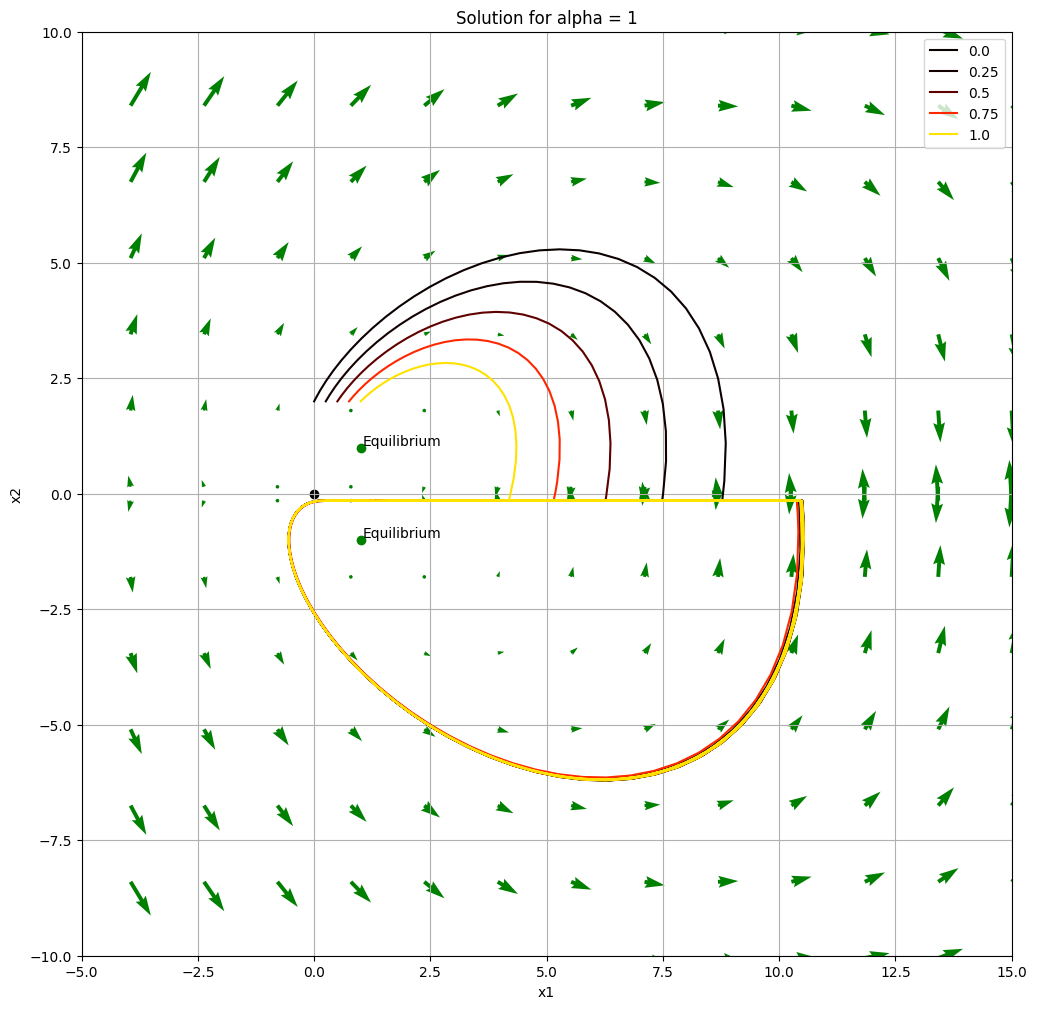
\includegraphics[width = 0.5\textwidth]{Images/initial conditions.png}
    \caption{A solution for $\ep = 0.15$ and $\alpha = 1$. There seems to be slight differences in orbit.}
    \label{png:initial conditions}
    \end{figure}

    \vspace{\floatsep}
    \clearpage


    My intuition for $\alpha = 0.5$ would be that the solution would shoot off into the negative $x_2$ direction forever. Coming back to observing only one solution, it seems this is only the case when I put my initial conditions exactly on the boundary line. If I put place my initial conditions in a nonzero distance from the $x_2$ axis, but still within $\ep$, the solution will be attracted by the system, and will be captured in orbit. I have added my plot for initial conditions equal $(0, 0)$ in Figure \ref{png:origin  conditions}, as well as the initial conditions $(0, 0.01)$ in Figure \ref{png:perturbation condition}.
    
    \jump
    \begin{figure}[!ht]
    \centering
    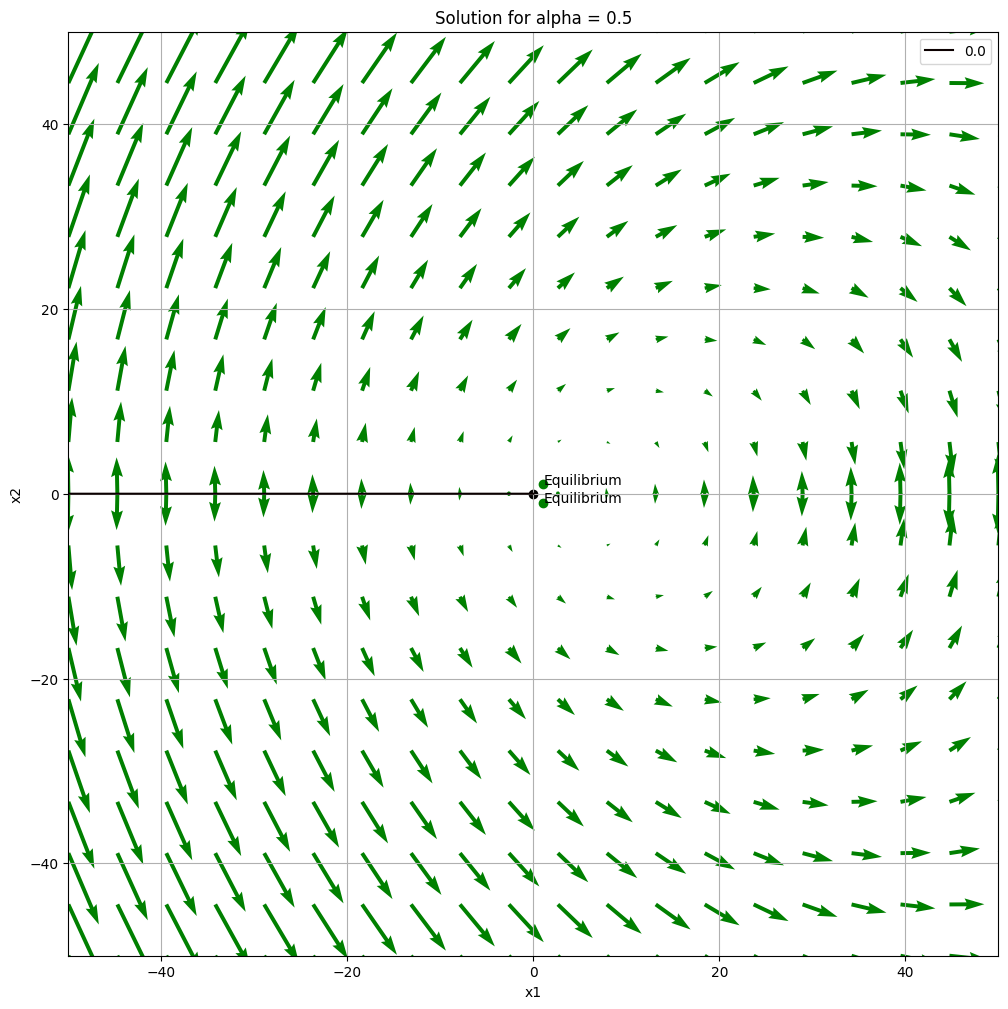
\includegraphics[width = 0.5\textwidth]{Images/origin conditions.png}
    \caption{A solution for $\ep = 0.05$ and $\alpha = 0.5$ and initial conditions at the origin. Note the solution shoots off to the left. I increased the limits of the plot to confirm this.}
    \label{png:origin conditions}
    \end{figure}

    \vspace{\floatsep}
    \clearpage

    \jump
    \begin{figure}[!ht]
    \centering
    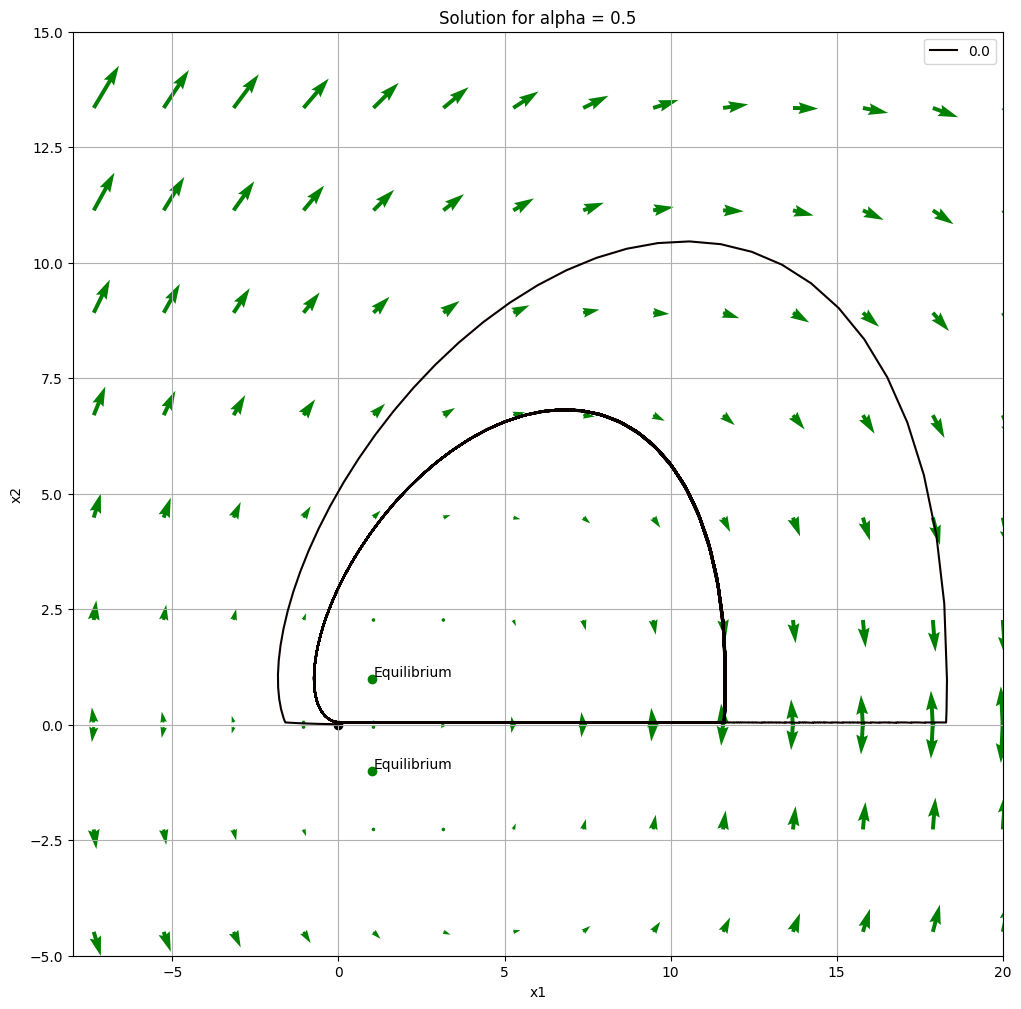
\includegraphics[width = 0.5\textwidth]{Images/perturbation conditions.png}
    \caption{A solution for $\ep = 0.05$ and $\alpha = 0.5$ and initial conditions $(0, 0.01)$. This is within $\ep$ distance of the $x_2$ axis. Note the first orbit is much larger than resulting orbits due to initial weak attraction.}
    \label{png:perturbation condition}
    \end{figure}

    \vspace{\floatsep}
    \clearpage
\end{solution}

\begin{lstlisting}
import numpy as np 
import matplotlib.pyplot as plt 
from scipy.integrate import solve_ivp
import matplotlib.cm as cm

#System definition
def xdot(y, t, alpha, eps):
    
    x1, x2 = y
    
    if x2 > eps:
        return [-1 + x2, x2 - x1]
    elif x2 < -eps:
        return [-1 - x2, x1 + x2]
    else:
        return [ alpha *(-1 + x2) + (1 - alpha) * (-1 - x2),
                 alpha *(x2 - x1) + (1 - alpha) * (x2 + x1)]

#define time range
timespan = (0., 500.)
#initial conditions
x0s = np.linspace(0, 1, 1)
y0 = 0.01
alpha = 0.5
eps = 0.05

colors = np.linspace(0, 1 / max(max(x0s), 1), 5)
fig, axs = plt.subplots(1, 1, figsize =(12, 12))
i = 0
for x0 in x0s:  
    initial_conditions = [x0, y0]
    #Getting numerical Solution
    sol = solve_ivp(lambda t, y: xdot(y, t, alpha, eps), t_span=timespan, y0=initial_conditions, max_step = 0.1)
    #Picking coords of solution 
    x, y = sol.y
    axs.plot(x, y, color = cm.hot(min(colors[i]**3, 0.7)), label = x0)
    i+=1
    
bound = 20 #Plotting bounds for x and y axis


#Adding a small buffer for which the boundary term will occupy
xpos, ypos= np.meshgrid(np.linspace(-bound, bound, 20), 
                   np.linspace(eps , bound, 10)) 
                   
xmin, ymin= np.meshgrid(np.linspace(-bound, bound, 20), 
                   np.linspace(-bound, -eps, 10))
                   
# Not plotting these, they're pretty messy         
#xbound, ybound = np.meshgrid(np.linspace(-bound, bound, 200),  
#                   np.linspace(-eps, eps, 4))


#Update vector fields
#Vector directions for f plus and f minus
uplus = -1 + ypos
vplus = ypos - xpos
umin = -1 - ymin
vmin = xmin + ymin
#ubound = alpha * uplus + (1 - alpha) * umin
#vbound = alpha * vplus + (1 - alpha) * vmin




# Plotting Vector Field
axs.quiver(xpos, ypos, uplus, vplus, color='g') 
axs.quiver(xmin, ymin, umin, vmin, color='g') 
#axs.quiver(xbound, ybound, ubound, vbound, color = 'r')
axs.set_title('Solution for alpha = {}'.format(alpha))
axs.grid(True)
axs.scatter([0], [0], color = 'k')
axs.scatter([1, 1], [1, -1], color = 'g')

axs.annotate("Equilibrium", (1.05, 1.05))
axs.annotate("Equilibrium", (1.05, -0.95))
#axs.annotate("Initial", (x0 - 1, y0 - 0.1))
#axs.annotate("Final", (x[-1] - 1, y[-1] + 0.5))

axs.set_xlabel("x1")
axs.set_ylabel("x2")
axs.legend()
# Setting x, y boundary limits 
plt.xlim(-8, bound) 
plt.ylim(-5, 15) 
  
# Show plot with grid 
plt.show() 

\end{lstlisting}
\end{document}